\subsection{数据采集模块}
\par 该模块以\texttt{Frame}类(见表\ref{table:Frame})为主体,它统一管理RGB-D相机和图像数据,图像数据每帧更新一次,组件图和时序图如图\ref{fig:component1}、图\ref{fig:sequence1}所示。

% \begin{figure}[htb]
% 	\centering
% 	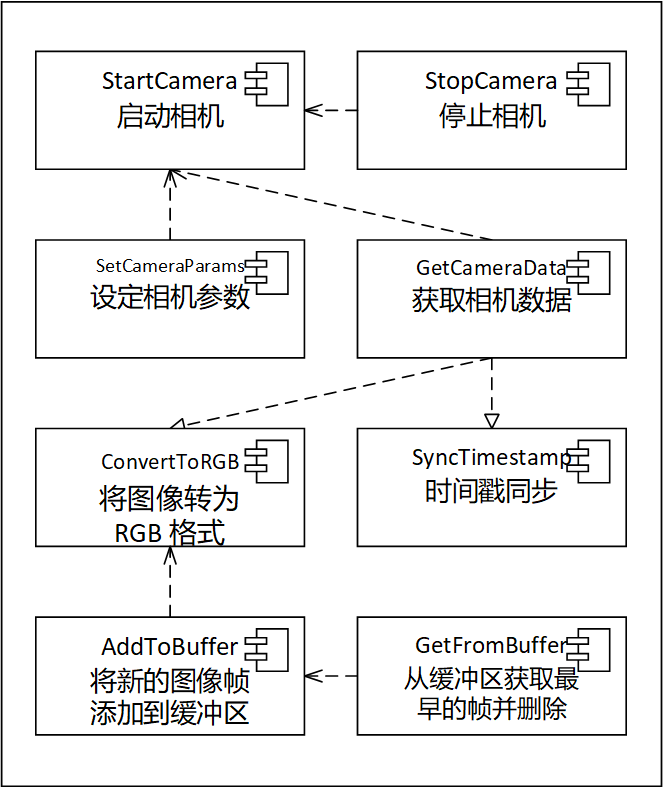
\includegraphics[width=0.7\textwidth]{figures/uml/component1.png}
% 	\caption{数据采集模块组件图}
% 	\label{fig:component1}
% \end{figure}

\begin{figure}[htb]
	\centering
	\begin{minipage}[t]{0.44\textwidth}
		\centering
		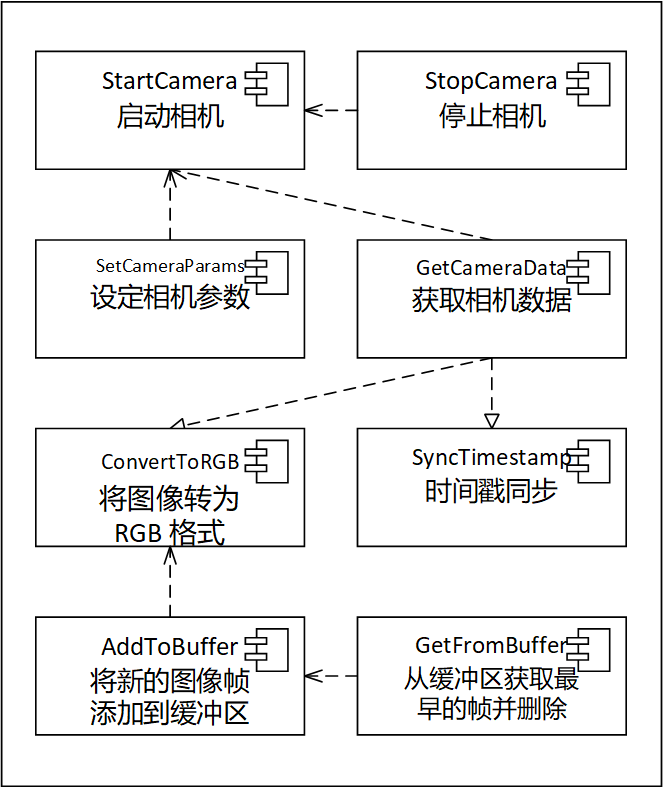
\includegraphics[height=7.5cm,keepaspectratio]{figures/uml/component1.png}
		\caption{数据采集模块组件图}
		\label{fig:component1}
	\end{minipage}
	\begin{minipage}[t]{0.51\textwidth}
		\centering
		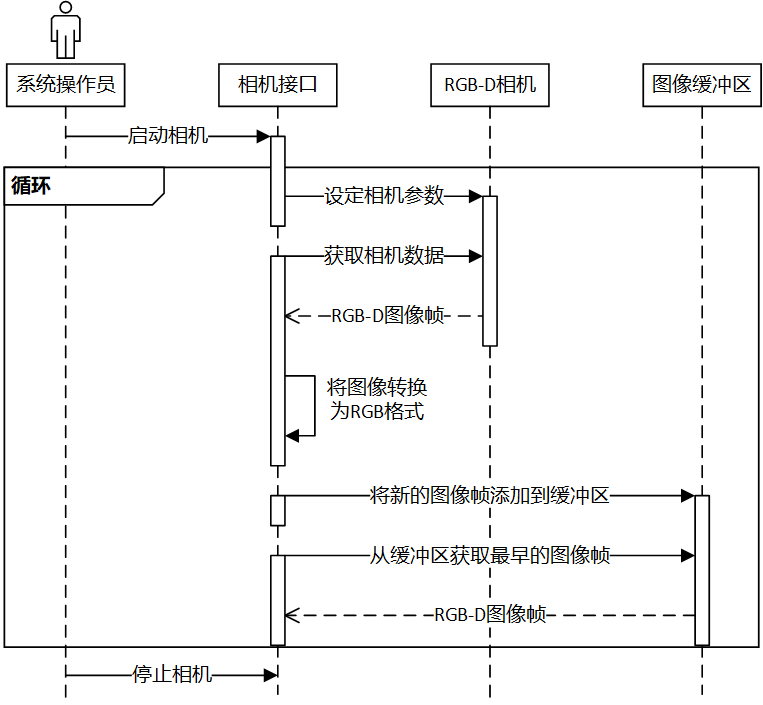
\includegraphics[height=7.5cm,keepaspectratio]{figures/uml/sequence1.png}
		\caption{数据采集模块时序图}
		\label{fig:sequence1}
	\end{minipage}
\end{figure}

\begin{table}[htb]
	\centering
	\caption{Frame类的主要成员和方法}
	\label{table:Frame}
	\begin{tabular}{|l|m{3.5cm}|m{3.5cm}|m{5cm}|}
		\hline
		                                           & \multicolumn{1}{c|}{名称}                         & \multicolumn{1}{c|}{类型}                       & \multicolumn{1}{c|}{功能}                 \\ \hline
		\multicolumn{1}{|c|}{\multirow{12}{*}{成员}} & \centering\arraybackslash current\_frame\_index & \centering\arraybackslash int                 & \centering\arraybackslash 当前帧的序号        \\ \cline{2-4}
		\multicolumn{1}{|c|}{}                     & \centering\arraybackslash pipeline              & \centering\arraybackslash rs2::pipeline       & \centering\arraybackslash RealSense相机对象 \\ \cline{2-4}
		\multicolumn{1}{|c|}{}                     & \centering\arraybackslash rgb\_width            & \centering\arraybackslash unsigned int        & \centering\arraybackslash RGB图像的宽度      \\ \cline{2-4}
		\multicolumn{1}{|c|}{}                     & \centering\arraybackslash rgb\_height           & \centering\arraybackslash unsigned int        & \centering\arraybackslash RGB图像的高度      \\ \cline{2-4}
		\multicolumn{1}{|c|}{}                     & \centering\arraybackslash depth\_width          & \centering\arraybackslash unsigned int        & \centering\arraybackslash 深度图像的宽度       \\ \cline{2-4}
		\multicolumn{1}{|c|}{}                     & \centering\arraybackslash depth\_height         & \centering\arraybackslash unsigned int        & \centering\arraybackslash 深度图像的高度       \\ \cline{2-4}
		\multicolumn{1}{|c|}{}                     & \centering\arraybackslash rgb\_image            & \centering\arraybackslash cv::Mat             & \centering\arraybackslash RGB图像         \\ \cline{2-4}
		\multicolumn{1}{|c|}{}                     & \centering\arraybackslash depth\_image          & \centering\arraybackslash cv::Mat             & \centering\arraybackslash 深度图像          \\ \cline{2-4}
		\multicolumn{1}{|c|}{}                     & \centering\arraybackslash semantic\_image       & \centering\arraybackslash cv::Mat             & \centering\arraybackslash 语义分割图像        \\ \cline{2-4}
		\multicolumn{1}{|c|}{}                     & \centering\arraybackslash rgb\_viewer           & \centering\arraybackslash Viewer              & \centering\arraybackslash RGB图像的位姿      \\ \cline{2-4}
		\multicolumn{1}{|c|}{}                     & \centering\arraybackslash depth\_viewer         & \centering\arraybackslash Viewer              & \centering\arraybackslash 深度图像的位姿       \\ \cline{2-4}
		\multicolumn{1}{|c|}{}                     & \centering\arraybackslash buffer                & \centering\arraybackslash queue          & \centering\arraybackslash 图像缓冲区         \\ \hline
		\multirow{14}{*}{方法}                       & \centering\arraybackslash StartCamera           & \centering\arraybackslash void                & \centering\arraybackslash 启动相机          \\ \cline{2-4}
		                                           & \centering\arraybackslash StopCamera            & \centering\arraybackslash void                & \centering\arraybackslash 停止相机          \\ \cline{2-4}
		                                           & \centering\arraybackslash SetCameraParams       & \centering\arraybackslash void                & \centering\arraybackslash 设定相机参数        \\ \cline{2-4}
		                                           & \centering\arraybackslash GetCameraData         & \centering\arraybackslash rs2::frameset       & \centering\arraybackslash 获取相机数据        \\ \cline{2-4}
		                                           & \centering\arraybackslash SyncTimestamp         & \centering\arraybackslash void                & \centering\arraybackslash 时间戳同步         \\ \cline{2-4}
		                                           & \centering\arraybackslash ConvertToRGB          & \centering\arraybackslash tuple          & \centering\arraybackslash 将图像转换为RGB格式   \\ \cline{2-4}
		                                           & \centering\arraybackslash AddToBuffer           & \centering\arraybackslash void                & \centering\arraybackslash 将新的图像帧添加到缓冲区  \\ \cline{2-4}
		                                           & \centering\arraybackslash GetFromBuffer         & \centering\arraybackslash tuple          & \centering\arraybackslash 从缓冲区获取最早的帧并删除 \\ \cline{2-4}
		                                           & \centering\arraybackslash AlignImage            & \centering\arraybackslash cv::Mat             & \centering\arraybackslash 对齐RGB图像和深度图像  \\ \cline{2-4}
		                                           & \centering\arraybackslash DenoiseImage          & \centering\arraybackslash cv::Mat             & \centering\arraybackslash 图像去噪与增强       \\ \cline{2-4}
		                                           & \centering\arraybackslash CropImage             & \centering\arraybackslash cv::Mat             & \centering\arraybackslash 裁剪图像的无效区域     \\ \cline{2-4}
		                                           & \centering\arraybackslash ResizeImage           & \centering\arraybackslash cv::Mat             & \centering\arraybackslash 图像缩放          \\ \cline{2-4}
		                                           & \centering\arraybackslash SegmentImage          & \centering\arraybackslash cv::Mat             & \centering\arraybackslash RGB图像语义分割     \\ \cline{2-4}
		                                           & \centering\arraybackslash NormalizeImage        & \centering\arraybackslash \_\_global\_\_ void & \centering\arraybackslash 图像格式转换和归一化    \\ \hline
	\end{tabular}
\end{table}

\par 首先,\texttt{StartCamera}通过调用Intel RealSense SDK 2.0的接口,启动Intel RealSense 相机。启动相机后,\texttt{SetCameraParams}设定相机的参数,包括图像分辨率、帧率、和深度距离。

\par 接下来,执行\texttt{GetCameraData}获取相机的数据。这个函数将返回一个包含RGB图像和深度图像的帧集。这里,通过调用\texttt{SyncTimestamp}确保RGB图像和深度图像的时间戳是同步的,它将根据相机型号,采用对应的硬件同步来对时间戳进行校正。

\par 获取和同步数据后,首先通过\texttt{ConvertToRGB}函数调用OpenCV接口,将图像转换成RGB格式。接着,通过\texttt{AddToBuffer}将图像添加到缓冲区,数据结构为\texttt{queue<tuple<cv::Mat, cv::Mat>>}。该函数首先检查当前缓冲区中存储的帧数是否达到了预设的上限。如果达到上限,将从缓冲区的前端(即最旧的帧)移除一帧数据。然后,将输入的RGB图像和深度图像包成一个元组,复制这些图像数据,再将该元组添加到缓冲区的末尾,即缓冲区的最新位置。

\par 相应地,\texttt{GetFromBuffer}的任务是从缓冲区获取最早的一帧数据。首先,它会检查缓冲区是否为空。如果缓冲区为空,那么它将抛出一个运行时错误,提示缓冲区无数据。如果缓冲区不为空,函数会从缓冲区的前端获取一个元组,并将其从缓冲区中删除。最后,返回该元组。

% \par 在数据采集模块中,数据流的控制以及异常处理与容错是非常重要的,这是通过\texttt{ControlDataFlow}函数来完成的。这个函数作为一个守护线程,负责协调数据采集和处理过程中的数据传递,确保数据的有效性、完整性和正确性。

\par 当数据采集的工作完成后,可以通过\texttt{StopCamera}函数停止相机。

\par 数据采集模块在整个系统中起着非常重要的角色。通过调用\texttt{Frame}类的部分函数,能够有效地管理和处理图像数据,为后续的任务提供高质量的数据输入。